\xchapter{Menções a software acadêmico de análise estática}
{Este capítulo apresenta uma revisão de literatura nas bases da ACM e IEEE em
busca de menções a projetos de software acadêmico de análise estática.}
\label{estudo2}

% macros LaTeX com os resultados encontrados no estudo
% dados do estudo1
\newcommand{\SoftwareCount}{60}
\newcommand{\SoftwareUrlNotAvailableCount}{15}
\newcommand{\SoftwareUrlAvailableCount}{45}
\newcommand{\SoftwareDownloadNotAvailableCount}{24}
\newcommand{\SoftwareDownloadAvailableCount}{36}
% dados do estudo2
\newcommand{\SearchACMCount}{438}
\newcommand{\SearchIEEECount}{459}
\newcommand{\SearchCount}{897}
\newcommand{\SearchUniqueCount}{806}
\newcommand{\ScreeningCount}{429}
\newcommand{\ScreeningUniqueCount}{416}
\newcommand{\CiteCount}{199}
\newcommand{\UseCount}{124}
\newcommand{\ContributeCount}{106}
\newcommand{\SearchUniqueMean}{13.4}
\newcommand{\ScreeningMean}{7.2}
\newcommand{\ScreeningUniqueMean}{6.9}
\newcommand{\MentionsStudyUm}{60}
\newcommand{\MentionsStudyDois}{47}
\newcommand{\SoftwareNotMentionedCount}{13}
\newcommand{\ContributeStudyDoisCount}{43}
\newcommand{\ContributeStudyDoisSoftware}{17}
% dados do estudo3
\newcommand{\ReleasesCount}{303}
\newcommand{\ReleasesAvailableCount}{211}
\newcommand{\ReleasesMetricsCount}{206}
\newcommand{\ProjectsWithReleasesCount}{35}
\newcommand{\ProjectsAnalizedCount}{24}
\newcommand{\ReleasesYearFirst}{2001}
\newcommand{\ReleasesYearLast}{2017}


Este estudo inspecionou \SearchUniqueCount \ artigos encontrados nas bases ACM
e IEEE através de uma revisão de literatura para caracterização de menções e
citações (formais e informais) a projetos de software acadêmico de análise
estática em relação a uso e contribuição.

A seção \ref{estudo2:introducao} contextualiza o estudo,
a seção \ref{estudo2:fundamentacao} apresenta os conceitos teóricos necessários para compreensão do trabalho,
a seção \ref{estudo2:definicao} descreve o objetivo e apresenta as questões de pesquisa,
a seção \ref{estudo2:planejamento} apresenta um planejamento do estudo,
as seções \ref{estudo2:preparacao} e \ref{estudo2:coleta} apresentam detalhes sobre a preparação e execução da coleta de dados,
as seções \ref{estudo2:analise} e \ref{estudo2:interpretacao} apresentam a análise e interpretação dos dados e
a seção \ref{estudo2:conclusoes} traça as conclusões finais deste estudo.

\section{Introdução e Motivação} \label{estudo2:introducao} % {{{

Os projetos de software desenvolvidos na academia sofrem de {\it
``dysfunctional chaotic churn''} \cite{howison2015understanding}.
Na prática, isso significa que há muitos projetos com características e
funcionalidades parecidas, com poucos usuários, com ciclos de vida curtos, e
encerrados quando o financiamento inicial termina, bem como, comunidades
desconectadas e paralelas, incompatibilidades entre projetos em um mesmo
domínio, e tentativas aparentemente não coordenadas de ``reiniciar'' tudo ({\it re-boots}). 

O desenvolvimento de sotware acadêmico é uma atividade que consome recursos
(tempo, dinheiro e atenção) e afeta a conduta da Ciência, tanto no geral como
em campos específicos, a colaboração no desenvolvimento destes projetos é vista
neste estudo como uma importante estratégia para lidar com o baixo orçamento
das pesquisas, bem como para mitigar os problemas do limitado tempo dos
cientistas e da alta rotatividade entre os grupos de pesquisa.

Esta estratégia de colaboração se torna especialmente interessante entre as
pesquisas da Engenharia de Software, onde, a princípio os cientistas possuem
acesso ao conhecimento e práticas necessárias para o trabalho em colaboração,
dessa forma, neste estudo investigamos como os projetos de software acadêmico
de análise estática são mencionados em publicações nas bases da ACM e IEEE e se
há colaboração entre eles.

% }}}

\section{Fundamentação} \label{estudo2:fundamentacao} % {{{

\subsection{Menção}

Menção neste estudo refere-se a qualquer ocorrência a nomes de projetos de
software acadêmico de análise estática, incluindo tanto citação formal, quanto
informal, a prática científica de citação formal entre publicações, amplamente
adotada e praticada entre cientistas de todas as áreas, não é realidade quando
se trata de artefatos digitais, como dados ou código, por exemplo.

Software é citado na literatura acadêmica, na maior parte das ocorrências, de
maneira informal, em notas de rodapé, seções de agradecimentos, em outras
seções ao longo do texto, usualmente se faz referência ao nome, ocasionalmente
cita-se o número da versão, e raramente usa-se citação formal.

% }}}

\section{Definição} \label{estudo2:definicao} % {{{

Quantas menções a projetos de software acadêmico de análise estática são
encontradas em publicações nas bases da ACM e IEEE? Quais são os tipos de
menções? Existe contribuição em código fonte aos projetos entre as publicações
encontradas?

\subsection{Definição do Objetivo}

\begin{description}
\item{\bf Objeto de estudo.} 
O objeto de estudo são projetos de software de análise estática publicados nas conferências ASE e SCAM.

\item{\bf Propósito.} 
O propósito deste estudo é caracterizar menções aos projetos.

\item{\bf Perspectiva.} 
A perspectiva considerada é a de cientista preocupado com o funcionamento do ecossistema de software acadêmico.

\item{\bf Foco de qualidade.} 
O principal aspecto de qualidade estudado é a contribuição ao ecossistema de software acadêmico de análise estática.

\item{\bf Contexto.} 
O estudo foi conduzido com publicações das bases ACM e IEEE.
\end{description}

\subsection{Sumário da Definição}

Analisar os \textit{projetos de software acadêmico de análise estática publicados nas conferências ASE e SCAM}
com o propósito de \textit{caracterizar menções}
com respeito a \textit{contribuição ao ecossistema de software acadêmico}
na perspectiva de \textit{cientistas}
no contexto de \textit{publicações nas bases ACM e IEEE}.

\subsection{Questões de Pesquisa}

Neste estudo as seguintes questões de pesquisa, a respeito dos projetos de
software acadêmico de análise estática, serão investigadas:

\newcommand{\EstudoDoisQuestaoUm}{Como os projetos de software acadêmico de
análise estática publicados nas conferências ASE e SCAM são mencionados em
publicações nas bases ACM e IEEE?}

\newcommand{\EstudoDoisQuestaoDois}{Os projetos de software acadêmico de
análise estática publicados nas conferências ASE e SCAM são utilizados
em publicações nas bases ACM e IEEE?}

\newcommand{\EstudoDoisQuestaoTres}{Os projetos de software acadêmico de
análise estática publicados nas conferências ASE e SCAM recebem contribuições
de código fonte em publicações nas bases ACM e IEEE?}

\begin{description}
  \item [Q1:] \EstudoDoisQuestaoUm
  \item [Q2:] \EstudoDoisQuestaoDois
  \item [Q3:] \EstudoDoisQuestaoTres
\end{description}

\subsection{Métricas}

Para responder às questões de pesquisas, as seguintes métricas serão usadas:

\begin{enumerate}
  \item Número de publicações nas bases ACM e IEEE mencionando projetos de
    software acadêmico de análise estática.
  \item Número de publicações nas bases ACM e IEEE mencionando uso de
    software acadêmico de análise estática.
  \item Número de publicações nas bases ACM e IEEE mencionando contribuição de
    código fonte a projetos de software acadêmico de análise estática.
\end{enumerate}

% }}}

\section{Planejamento do Estudo} \label{estudo2:planejamento} % {{{

O estudo foi realizado a partir de uma revisão de literatura nas bases ACM e
IEEE em busca de menções aos \SoftwareCount \ projetos de software acadêmico de
análise estática selecionados no Capítulo \ref{estudo1}, um esquema de
caracterização para classificação das menções emergiu dessa revisão, os artigos
foram então inspecionados e as menções encontradas foram classificadas segundo
este esquema.

A revisão de literatura foi organizada em quatro passos, detalhados a seguir.

\subsection{Passo 1: Busca}

Este passo teve como objetivo encontrar artigos nas bases
ACM\footnote{\url{http://dl.acm.org}} e
IEEE\footnote{\url{http://ieeexplore.ieee.org}} a partir das características
dos projetos de software acadêmico de análise estática.
As duas bases serão pesquisadas através de strings de busca previamente
elaboradas para cada um dos projetos.

A elaboração das strings deve ser realizada com o apoio dos dados já coletados
e disponíveis para cada projeto de software acadêmico, por exemplo, nome,
descrição, autores, URL, entre outros dados. Este processo de criação das
strings é realizado de maneira incremental e iterativa, iniciando por uma busca
utilizando apenas o nome do projeto, avaliando os resultados, inspecionando o
título dos artigos, refinando as strings e repetindo todo o processo até
atingir resultados dentro dos critérios desejados.

Estes critérios são definidos principalmente pelo
número de resultados obtidos na busca,
sabemos, por experiência prática, que o número de referências a cada projeto na
literatura acadêmica não chega a casa da centena, dessa forma, o critério de
aceitação para parada do processo de elaboração e refinamento das strings é
quando os resultados apresentem um número inferior ou próximo a esta realidade.

A elaboração das strings e a busca com a versão final será
realizada manualmente usando a busca avançada dos sites das bases pesquisadas,
representadas nas Figuras \ref{advanced-search-acm} e
\ref{advanced-search-ieee} com destaque para os campos e elementos de formulário
utilizados. É importante destacar que durante a busca na
base IEEE -- Figura \ref{advanced-search-ieee} -- é necessário marcar a opção {\it Full Text \& Metadata} para que a
busca considere tanto os metadados quanto o conteúdo dos artigos.

\begin{figure}[h]
  \center
  \frame{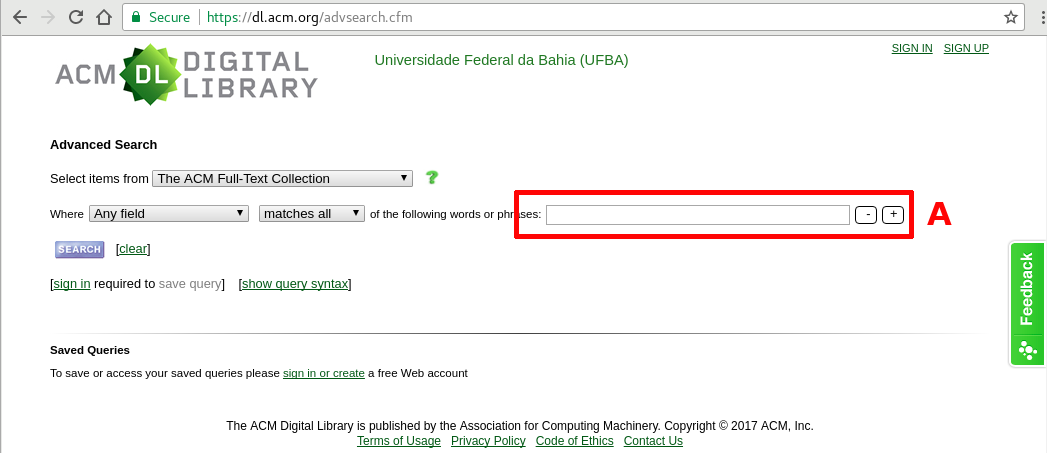
\includegraphics[scale=0.4]{imagens/advanced-search-acm.png}}
  \caption{Captura de tela da busca avançada da base ACM com destaque para (A) campo de entrada da string de busca.}
  \label{advanced-search-acm}
\end{figure}

\begin{figure}[h]
  \center
  \frame{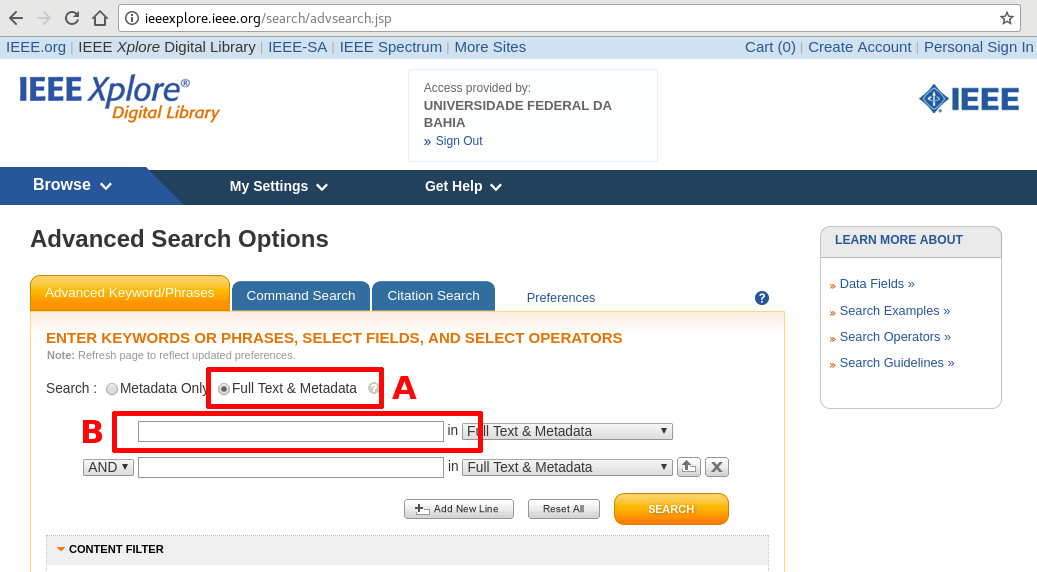
\includegraphics[scale=0.4]{imagens/advanced-search-ieee.png}}
  \caption{Captura de tela da busca avançada da base IEEE com destaque para (A) opção de busca completa e (B) campo de entrada da string de busca.}
  \label{advanced-search-ieee}
\end{figure}

O resultado da busca final de cada projeto em cada base deve ser exportado e
copiado localmente em formato BibTeX, ambas as bases exportam os resultados
neste formato. O resultado final da busca de todos os projetos serão combinados
e agregados num resultado único sem duplicação de resultados contendo os
metadados de todos os artigos, sem repetição.

Este resultado final, além de eliminar a duplicação de resultados, será a base
para a definição de uma identificação única para cada artigo encontrado, esta
identificação será utilizada nos próximos passos para relacionar os projetos
aos artigos através das menções encontradas. Por fim, será feito o download de cada
artigo em formato pdf para inspeção manual na etapa seguinte.

\subsection{Passo 2: Triagem}

Neste passo selecionamos os artigos relevantes para cada projeto entre os
resultados da busca realizada no passo anterior, a seleção é realizada através
de inspeção manual de cada artigo entre os resultados de cada projeto. O
critério de inclusão para a seleção dos artigos relevantes é a simples
ocorrência do nome do projeto no artigo.

Cada artigo entre os resultados de cada projeto deverá ser identificado como
relevante para o projeto caso o critério de inclusão seja satisfeito durante a
inspeção manual do artigo. Ao final deste passo teremos para cada projeto
de software um conjunto de artigos identificados como relevantes fazendo
menção ao nome do projeto.

\subsection{Passo 3: Keywording}

Neste passo será criado um esquema de codificação para caracterização das
menções, o esquema é criado a partir da identificação do contexto em que os
projetos são mencionados, para cada menção toma-se nota sobre como o projeto de
software é mencionado no artigo.

As notas são comentários livres descrevendo as menções encontradas no artigo
sobre um determinado software, um artigo científico pode mencionar um software
diversas vezes, de diversas formas, desde uma simples menção nos trabalhos
relacionados até uma grande contribuição ao software.

O conjunto final de todas as anotações são agrupadas e analisadas em conjunto
para definição do esquema de codificação para caracterização das menções. Este
esquema deve ser construído com o objetivo de agrupar e caracterizar os tipos
de menção encontrados para cada projeto de software em termos da contribuição
que a menção traz ao ecossistema de software daquele projeto acadêmico.

%, cada
%menção representa uma entrada em forma de contribução ao ecossistema, seja
%fazendo o projeto de software ser visível na literatura acadêmica, seja com
%contribuição direta em código ao projeto.

\subsection{Passo 4: Extração}

Neste último passo da revisão de literatura utiliza-se o esquema de codificação
para caracterização de menções criado no passo anterior para classificar as
menções de cada projeto de software encontradas nos artigos relevantes
selecionados no Passo 2: Triagem.

Para cada artigo mencionando um certo projeto de software será atribuído uma
informação indicando o tipo de menção entre as opções do esquema de codificação
para caracterização das menções.

Ao final da revisão de literatura teremos para cada projeto de software um
conjunto de artigos relevantes mencionando o software, com indicação do tipo de menção
através do esquema de codificação para caracterização de menções elaboradas no Passo 3: Keywording.

% }}}

\section{Preparação} \label{estudo2:preparacao} % {{{

Nesta seção apresentamos a preparação do estudo para a realização da coleta de
dados, incluindo a definição de arquivos e formatos de armazenamento, bem como
a implementação de scripts para coleta, análise e transformação.
A Figura \ref{estudo2-fluxograma} apresenta uma visão geral da solução adotada
e da relação entre os passos da revisão de literatura, detalhados a seguir.

\begin{figure}[h]
  \center
  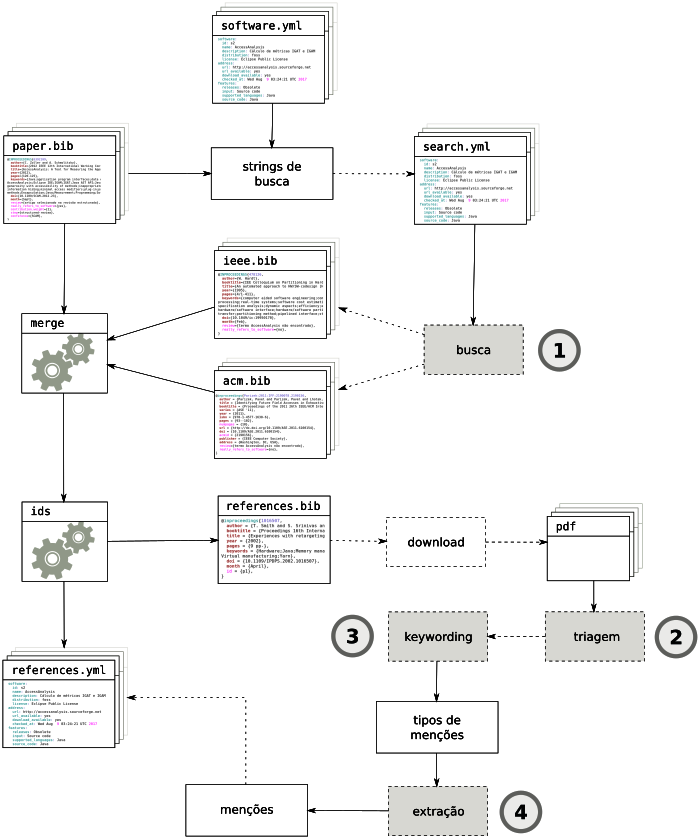
\includegraphics[scale=0.35]{imagens/estudo2-fluxograma.png}
  \caption{Fluxo de coleta, análise e transformação dos dados.}
  \label{estudo2-fluxograma}
\end{figure}

%Definimos em linhas gerais utilizar arquivos em texto plano para armazenar
%os dados coletados visando a facilidade e transparência ao acesso aos dados
%por

\subsection{Passo 1: Busca}

Seguindo o planejamento descrito na seção \ref{estudo2:planejamento} criamos as
strings de busca e as registramos nos arquivos \texttt{search.yml} de cada
projeto, este arquivo irá registrar também o número de resultados e a data de
execução da busca. A Listagem \ref{search-yml} apresenta um exemplo deste
arquivo com campos utilizados para registrar os resultados da busca.

\begin{lstlisting}[
caption={Arquivo search.yml.},
label={search-yml},
frame=single,
numbers=left
]
  acm:
    string:
    searched_at:
    results:
  ieee:
    string:
    searched_at:
    results:
\end{lstlisting}

Além deste arquivo, será criado também para cada projeto os arquivos
\texttt{acm.bib} e \texttt{ieee.bib} para armazenar os dados dos artigos
retornados pela busca. Estes dados, de todos os projetos, serão agregados no
arquivo \texttt{documents/references.bib} e identificados com
o campo \texttt{id} recebendo valores no formato \texttt{p + NÚMERO},
exemplo, \texttt{p1}, \texttt{p2}, \texttt{p3}, ..., \texttt{p806}.

Foi implementado o script \texttt{bin/ids} para automatizar a
definição deste novo campo para cada artigo, ele recebe como entrada um arquivo
no formato BibTeX e gera sequencialmente o campo \texttt{id} para cada item.

\subsection{Passo 2: Triagem}

Definimos a estrutura do arquivo \texttt{references.yml} onde será registrada a
informação dos artigos relevantes para cada projeto, a Listagem
\ref{references-yml} apresenta um exemplo deste arquivo e de sua estrutura.

\begin{lstlisting}[
caption={Arquivo references.yml.},
label={references-yml},
frame=single,
numbers=left
]
  p1:
    review:
    is_software_mentioned:
  p2:
    review:
    is_software_mentioned:
  p3:
    review:
    is_software_mentioned:
\end{lstlisting}

Em paralelo a definição deste arquivo, implementamos um mecanismo de templates,
através dos scripts \texttt{bin/cache} e \texttt{bin/render}, para criação
automática desses arquivos para cada projeto, este mecanismo de templates será
utilizado em outros pontos de estudo para automatizar e produzir documentos a
partir dos dados coletados, este mecanismo é apresentado em resumo na Figura
\ref{template-fluxograma}.

\begin{figure}[h]
  \center
  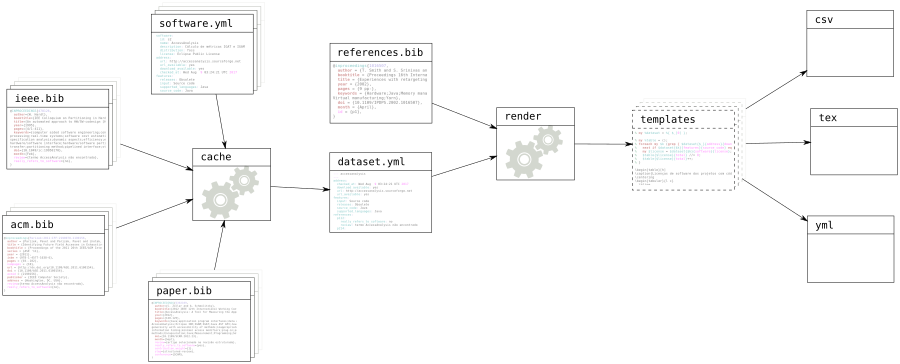
\includegraphics[scale=0.3]{imagens/template-fluxograma.png}
  \caption{Mecanismo de template para transformar dados em documentos para visualização e análise.}
  \label{template-fluxograma}
\end{figure}

%  \item[\texttt{bin/merge}]
%    Agrega os arquivos \texttt{acm.bib}, \texttt{ieee.bib} e \texttt{paper.bib}
%    de cada projeto em um único arquivo no formato BibTeX removendo
%    duplicidades dos resultados.

O script \texttt{bin/cache} cria o arquivo \texttt{cache/dataset.yml} ao
agregar todos os dados coletados de todos os projetos a partir dos arquivos
\texttt{software.yml}, \texttt{acm.bib}, \texttt{ieee.bib}, \texttt{paper.bib},
\texttt{references.yml} e \texttt{search.yml}.
O script \texttt{bin/render} lê este arquivo \texttt{cache/dataset.yml},
carrega os dados em memória e passa estes dados como parâmetro para os arquivos
templates.

\subsection{Passo 3: Keywording}

Adicionamos aos arquivos \texttt{references.yml} um novo campo para coletar o
tipo de menção feita em cada artigo aos projetos, \texttt{mention\_type}, este
campo assume um dos valores do esquema de classificação criado neste passo.

\subsection{Passo 4: Extração}

Implementamos arquivos de template para representar os dados coletados em
outros formatos para visualização e análise, incluindo documentos em formatos
CSV, Markdown e \LaTeX. Alguns destes documentos são incluídos automaticamente
neste texto.

% }}}

\section{Coleta de dados} \label{estudo2:coleta} % {{{

Seguindo o planejamento e preparação descritos nas seções
\ref{estudo2:planejamento} e \ref{estudo2:preparacao} iniciamos a coleta dos
dados através da revisão de literatura, apresentado em resumo na Figura \ref{estudo2-revisao-literatura}.

\begin{figure}[h]
  \center
  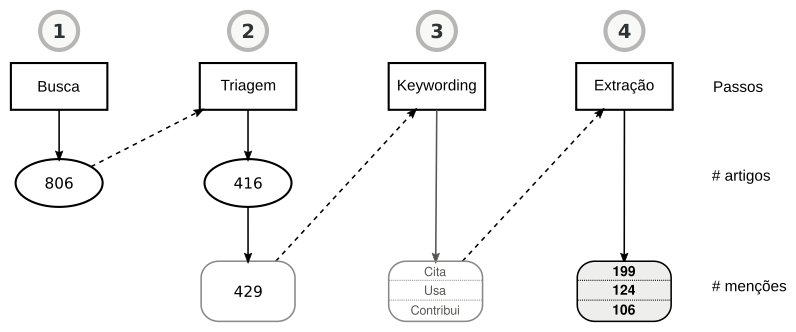
\includegraphics[scale=0.35]{imagens/estudo2-revisao-literatura.png}
  \caption{Passos da revisão de literatura realizada nas bases ACM e IEEE.}
  \label{estudo2-revisao-literatura}
\end{figure}


\subsection{Passo 1: Busca}

A busca de todos os projetos retornou \SearchCount \ resultados,
\SearchACMCount \ na base ACM e \SearchIEEECount \ na base IEEE.
Estes resultados incluem duplicação de artigos, ou seja,
um mesmo artigo encontrado nas duas bases, ou, um mesmo artigo
encontrado em relação a mais de um projeto, dentre o resultado total.

Ao remover as duplicidades temos um conjunto de \SearchUniqueCount \ artigos
únicos.  A Tabela \ref{search-table} apresenta o total de resultados para cada
um dos projetos pesquisados, a coluna {\bf Total} inclui os artigos do arquivo
\texttt{paper.bib} e apresenta apenas resultados únicos.

\begin{longtable}{ l c c c | l c c c }
\caption{Número de resultados obtidos na busca de cada projeto de software.}
\label{search-table} \\
  \hline
  \hhline{ l c c c | l c c c |}
  \endfirsthead
  \hhline{ l c c c | l c c c |}
  \hline
   \multirow{2}{*}{\textbf{ID}} & \multicolumn{2}{c}{{\bf Busca}} & \multirow{2}{*}{\textbf{Total}} & \multirow{2}{*}{\textbf{ID}} & \multicolumn{2}{c}{{\bf Busca}} & \multirow{2}{*}{\textbf{Total}} \\
   & \textbf{ACM} & \textbf{IEEE} & & & \textbf{ACM} & \textbf{IEEE} & \\
  \hline
  \hhline{ l c c c | l c c c |}
  \endhead
  \hhline{----|----}
  \multicolumn{8}{c}{continua na próxima página} \\
  \hhline{----|----} \endfoot
  \hhline{----|----} \endlastfoot
   \multirow{2}{*}{\textbf{ID}} & \multicolumn{2}{c}{{\bf Busca}} & \multirow{2}{*}{\textbf{Total}} & \multirow{2}{*}{\textbf{ID}} & \multicolumn{2}{c}{{\bf Busca}} & \multirow{2}{*}{\textbf{Total}} \\
   & \textbf{ACM} & \textbf{IEEE} & & & \textbf{ACM} & \textbf{IEEE} & \\
  \hline
\texttt{s1} & 11 & 26 & 38 & \texttt{s32} & 19 & 18 & 32 \\
\texttt{s2} & 5 & 3 & 8 & \texttt{s33} & 3 & 3 & 5 \\
\texttt{s3} & 10 & 6 & 15 & \texttt{s34} & 1 & 3 & 4 \\
\texttt{s4} & 4 & 6 & 9 & \texttt{s35} & 2 & 1 & 2 \\
\texttt{s5} & 4 & 3 & 6 & \texttt{s36} & 17 & 20 & 34 \\
\texttt{s6} & 6 & 2 & 7 & \texttt{s37} & 2 & 5 & 7 \\
\texttt{s7} & 16 & 9 & 25 & \texttt{s38} & 29 & 20 & 42 \\
\texttt{s8} & 7 & 7 & 13 & \texttt{s39} & 3 & 10 & 11 \\
\texttt{s9} & 4 & 4 & 8 & \texttt{s40} & 3 & 8 & 11 \\
\texttt{s10} & 12 & 4 & 14 & \texttt{s41} & - & - & 1 \\
\texttt{s11} & 2 & 2 & 3 & \texttt{s42} & 1 & 4 & 5 \\
\texttt{s12} & 6 & 1 & 6 & \texttt{s43} & - & 2 & 2 \\
\texttt{s13} & 6 & 3 & 9 & \texttt{s44} & 3 & 1 & 3 \\
\texttt{s14} & 1 & 1 & 2 & \texttt{s45} & 5 & 10 & 14 \\
\texttt{s15} & 15 & 4 & 16 & \texttt{s46} & 16 & 12 & 24 \\
\texttt{s17} & - & 1 & 1 & \texttt{s47} & 6 & 7 & 13 \\
\texttt{s16} & 1 & 4 & 5 & \texttt{s48} & 3 & 2 & 4 \\
\texttt{s18} & 23 & 24 & 47 & \texttt{s49} & 1 & 4 & 5 \\
\texttt{s19} & 20 & 30 & 45 & \texttt{s50} & 1 & 1 & 2 \\
\texttt{s20} & 7 & 3 & 10 & \texttt{s51} & 2 & 5 & 7 \\
\texttt{s21} & 1 & 3 & 3 & \texttt{s52} & 9 & 34 & 41 \\
\texttt{s22} & 4 & 4 & 5 & \texttt{s53} & 10 & 5 & 13 \\
\texttt{s23} & 2 & 11 & 12 & \texttt{s54} & 2 & 2 & 4 \\
\texttt{s24} & - & - & 1 & \texttt{s55} & 3 & 8 & 12 \\
\texttt{s25} & 20 & 17 & 34 & \texttt{s56} & 23 & 21 & 38 \\
\texttt{s26} & 5 & 2 & 7 & \texttt{s57} & 4 & 6 & 8 \\
\texttt{s27} & 2 & 4 & 5 & \texttt{s58} & 8 & 4 & 11 \\
\texttt{s28} & 26 & 24 & 50 & \texttt{s59} & 25 & 12 & 36 \\
\texttt{s29} & 11 & 5 & 15 & \texttt{s60} & - & 7 & 7 \\
\texttt{s30} & 4 & 9 & 10 & \texttt{{\bf Média}} & {\bf 7.3} & {\bf 7.7} & {\bf 13.8} \\
\texttt{s31} & 2 & 2 & 3 & \texttt{{\bf Total}} & {\bf 438} & {\bf 459} & {\bf 830} \\
\end{longtable}


\subsection{Passo 2: Triagem}

Os \SearchUniqueCount \ artigos foram inspecionados em busca de menções aos
projetos de software, encontramos \ScreeningCount \ menções entre
\ScreeningUniqueCount \ artigos.
Alguns projetos de software possui nomes comuns que foram encontrados nos
artigos mas não faziam referencia ao software, em alguns casos os nomes
apareciam em fórmulas matemáticas ou como parte do texto em contextos não
relacionados ao projeto.

A Figura \ref{screenshot-paper-p148-2ls} apresenta um destes casos, o nome do
projeto \texttt{s1} (2LS) foi encontrado no artigo \texttt{p148} (Statistical
Design Framework of Submicron Flip-Flop Circuits Considering Process
Variations) num contexto sem relação alguma com o projeto em sí.

\begin{figure}[h]
  \center
  \frame{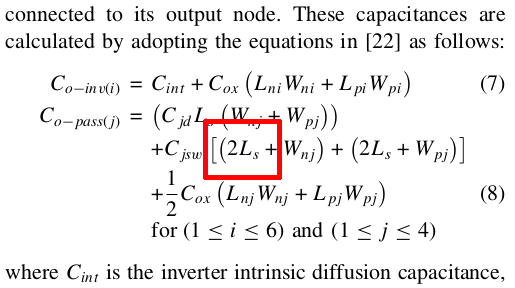
\includegraphics[scale=0.45]{imagens/screenshot-paper-p148-2ls.png}}
  \caption{Exemplo de ocorrencia do nome do projeto de software em fórmula matemática.}
  \label{screenshot-paper-p148-2ls}
\end{figure}

Ao final da triagem temos, para cada projeto, um conjunto de artigos que de
fato mencionam o software, sem ainda caracterizar o tipo de menção.

\subsection{Passo 3: Keywording}

A anotação de cada uma das \ScreeningCount \ menções foram analisadas e o
esquema para caracterização foi criado com três valores distintos indicando o
nível de contribuição da menção ao ecossistema de software do projeto,
apresentados na Tabela \ref{esquema-de-mencao}.

\begin{table}[h]
\caption{Esquema para classificação de menções aos projetos software acadêmico.}
\centering
\begin{tabular}{ l p{10cm} }
  \hline
  Tipo de menção           & Explicação \\
  \hline
  Cita      & É o mesmo artigo selecionado em \texttt{paper.bib} (artigo com ``mesmo'' conteúdo publicado na ``mesma'' época); Descreve o software; Menciona o software numa tabela com outros, classifica, cita como exemplo; Menciona em trabalhos relacionados ou em trabalhos futuros. \\
  Usa       & Avalia ou caracteriza o software; Usa para coleta ou análise de dados; Usa como objeto de estudo; Usa o software como parte de uma solução, implementação, etc; Cria um software derivado sem disponibilizar as contribuições. \\
  Contribui & Contribuição inicial publicando o software; Refatora o software; Abre o código de um software que antes era código fechado; Contribuição em código fonte; Extende o software; Integra o software a outros sistemas, formatos de entrada/saída ou APIs; Implementa parte do software em outro projeto e compara resultados. \\
  \hline
\end{tabular}
\label{esquema-de-mencao}
\end{table}

\subsection{Passo 4: Extração}

A partir do esquema para caracterização das menções coletamos os valores
assumindo um dos valores da Tabela \ref{esquema-de-mencao}, encontramos
\CiteCount \ menções do tipo Cita, \UseCount \ menções do tipo Usa e
\ContributeCount \ menções do tipo Contribui. Estes dados são
apresentados em resumo na Tabela \ref{mentions-table}.

\begin{longtable}{ l c c c c | l c c c c }
\caption{Número de menções por tipo para cada projeto.}
\label{mentions-table} \\
  \hline
  \hhline{ l c c c c | l c c c c |}
  \endfirsthead
  \hhline{ l c c c c | l c c c c |}
  \hline
   \multirow{2}{*}{\textbf{ID}} & \multicolumn{3}{c}{{\bf Menções}} & \multirow{2}{*}{\textbf{Total}} & \multirow{2}{*}{\textbf{ID}} & \multicolumn{3}{c}{{\bf Menções}} & \multirow{2}{*}{\textbf{Total}} \\
   & \textbf{Cita} & \textbf{Usa} & \textbf{Contribui} & & & \textbf{Cita} & \textbf{Usa} & \textbf{Contribui} & \\
  \hline
  \hhline{ l c c c c | l c c c c |}
  \endhead
  \hhline{-----|-----}
  \multicolumn{10}{c}{continua na próxima página} \\
  \hhline{-----|-----} \endfoot
  \hhline{-----|-----} \endlastfoot
   \multirow{2}{*}{\textbf{ID}} & \multicolumn{3}{c}{{\bf Menções}} & \multirow{2}{*}{\textbf{Total}} & \multirow{2}{*}{\textbf{ID}} & \multicolumn{3}{c}{{\bf Menções}} & \multirow{2}{*}{\textbf{Total}} \\
   & \textbf{Cita} & \textbf{Usa} & \textbf{Contribui} & & & \textbf{Cita} & \textbf{Usa} & \textbf{Contribui} & \\
  \hline
\texttt{s1} & - & - & 1 & 1 & \texttt{s32} & 8 & - & 6 & 14 \\
\texttt{s2} & 1 & - & 1 & 2 & \texttt{s33} & 2 & 2 & 1 & 5 \\
\texttt{s3} & 3 & - & 1 & 4 & \texttt{s34} & 1 & - & 1 & 2 \\
\texttt{s4} & 4 & 3 & 2 & 9 & \texttt{s35} & - & - & 1 & 1 \\
\texttt{s5} & 2 & - & 3 & 5 & \texttt{s36} & 1 & - & 1 & 2 \\
\texttt{s6} & 4 & - & 1 & 5 & \texttt{s37} & 3 & 1 & 3 & 7 \\
\texttt{s7} & 9 & - & 1 & 10 & \texttt{s38} & 17 & - & 1 & 18 \\
\texttt{s8} & 3 & 1 & 2 & 6 & \texttt{s39} & 1 & - & 1 & 2 \\
\texttt{s9} & - & - & 5 & 5 & \texttt{s40} & 1 & 5 & 3 & 9 \\
\texttt{s10} & 1 & 2 & 2 & 5 & \texttt{s41} & - & - & 1 & 1 \\
\texttt{s11} & 2 & - & 1 & 3 & \texttt{s42} & - & - & 1 & 1 \\
\texttt{s12} & 1 & - & 1 & 2 & \texttt{s43} & - & - & 2 & 2 \\
\texttt{s13} & - & - & 1 & 1 & \texttt{s44} & 1 & - & 1 & 2 \\
\texttt{s14} & 1 & - & 1 & 2 & \texttt{s45} & - & - & 2 & 2 \\
\texttt{s15} & 4 & - & 1 & 5 & \texttt{s46} & 9 & 3 & 1 & 13 \\
\texttt{s17} & - & - & 1 & 1 & \texttt{s47} & - & - & 1 & 1 \\
\texttt{s16} & 1 & 1 & 2 & 4 & \texttt{s48} & 1 & - & 1 & 2 \\
\texttt{s18} & - & 1 & 1 & 2 & \texttt{s49} & 1 & 2 & 2 & 5 \\
\texttt{s19} & 14 & 18 & 8 & 40 & \texttt{s50} & - & - & 1 & 1 \\
\texttt{s20} & - & - & 1 & 1 & \texttt{s51} & 1 & 2 & 1 & 4 \\
\texttt{s21} & - & - & 1 & 1 & \texttt{s52} & 14 & 23 & 3 & 40 \\
\texttt{s22} & 2 & - & 1 & 3 & \texttt{s53} & 1 & 2 & 1 & 4 \\
\texttt{s23} & 3 & 2 & 3 & 8 & \texttt{s54} & 1 & 1 & 1 & 3 \\
\texttt{s24} & - & - & 1 & 1 & \texttt{s55} & - & - & 1 & 1 \\
\texttt{s25} & 5 & 10 & 4 & 19 & \texttt{s56} & 15 & 5 & 1 & 21 \\
\texttt{s26} & 3 & 2 & 2 & 7 & \texttt{s57} & 4 & - & 1 & 5 \\
\texttt{s27} & - & 2 & 1 & 3 & \texttt{s58} & 5 & 5 & 1 & 11 \\
\texttt{s28} & 22 & 14 & 4 & 40 & \texttt{s59} & 16 & 10 & 7 & 33 \\
\texttt{s29} & 5 & 1 & 1 & 7 & \texttt{s60} & 4 & - & 1 & 5 \\
\texttt{s30} & 2 & 5 & 1 & 8 & \texttt{{\bf Média}} & {\bf 3.3} & {\bf 2.1} & {\bf 1.8} & {\bf 7.2} \\
\texttt{s31} & - & 1 & 1 & 2 & \texttt{{\bf Total}} & {\bf 199} & {\bf 124} & {\bf 106} & {\bf 429} \\
\end{longtable}


É importante lembrar que as menções do tipo Contribui incluem os artigos
selecionados no arquivo \texttt{paper.bib}, independente de terem sido
encontrados na busca das bases ACM e IEEE.

% }}}

% Raw results from the analysis
\section{Análise dos Dados} \label{estudo2:analise} % {{{

Dados de \SoftwareCount \ projetos desenvolvidos e publicados na literatura
acadêmica de Engenharia de Software, informações sobre diversas formas de
menção ao nome destes projetos, \ScreeningUniqueCount \ artigos distintos
encontrados nas bases ACM e IEEE mencionando estes projetos.

\subsection{Passo 1: Busca}

A busca nas bases ACM e IEEE retornou uma média de \SearchUniqueMean \ artigos
por projeto. Os projetos \texttt{s24} (GUIZMO) e \texttt{s41} (protopurity)
não foram encontrados em nenhuma das bases.
Os projetos \texttt{s17} (e-munity), \texttt{s43} (PtYasm) e \texttt{s60} (XOgastan)
não foram encontrados na base ACM.

Entre os projetos com resultados acima da média a maior parte está disponível
para download, 11 com acesso e 7 sem acesso.  Entre os projetos com resultados
abaixo da média, 25 está disponível para download e apenas 16 não estão
disponíveis.

%projetos com resultado da busca acima da média
% resultados  acesso
% s1  38      s
% s3  15      n
% s7  25      s
% s10 14      s
% s15 16      n
% s18 47      s
% s19 45      n
% s25 34      s
% s28 50      s
% s29 15      s
% s32 32      s
% s36 34      n
% s38 42      n
% s45 14      n
% s46 24      s
% s52 41      s
% s56 38      n
% s59 36      s
% s = 11
% n = 7

%projetos com resultado da busca abaixo da média
%resultados acesso
%s2  8      s
%s4  9      n
%s5  6      n
%s6  7      s
%s8  13     s
%s9  8      n
%s11 3      n
%s12 6      s
%s13 9      n
%s14 2      s
%s16 5      s
%s17 1      s
%s20 10     n
%s21 3      s
%s22 5      s
%s23 12     n
%s24 1      s
%s26 7      s
%s27 5      s
%s30 10     n
%s31 3      n
%s33 5      s
%s34 4      s
%s35 2      s
%s37 7      s
%s39 11     n
%s40 11     s
%s41 1      s
%s42 5      s
%s43 2      s
%s44 3      n
%s48 4      n
%s49 5      n
%s50 2      s
%s51 7      s
%s53 13     n
%s54 4      s
%s55 12     s
%s57 8      n
%s58 11     s
%s60 7      n

\subsection{Passo 2: Triagem}

Entre os resultados da busca apenas 51\% dos artigos são relevantes e fazem
menção aos projetos. Numa média de \ScreeningUniqueMean \ artigos por projeto
e \ScreeningMean \ menções por projeto.

Entre os projetos com menções acima da média, 9 estão disponíveis para download
e 6 não estão disponíveis, entre os projetos com menções abaixo da média, 25
possuem download disponível e 20 não.

% acima da média de menções
%          acesso
%s4  = 9   n
%s7  = 10  s
%s19 = 40  n
%s23 = 8   n
%s25 = 19  s
%s28 = 40  s
%s30 = 8   n
%s32 = 14  s
%s38 = 18  n
%s40 = 9   s
%s46 = 13  s
%s52 = 40  s
%s56 = 21  n
%s58 = 11  s
%s59 = 33  s

% abaixo da média de menções
%         acesso
%s1  = 1  s
%s2  = 2  s
%s3  = 4  n
%s5  = 5  n
%s6  = 5  s
%s8  = 6  s
%s9  = 5  n
%s10 = 5  s
%s11 = 3  n
%s12 = 2  s
%s13 = 1  n
%s14 = 2  s
%s15 = 5  n
%s16 = 4  n
%s17 = 1  s
%s18 = 2  s
%s20 = 1  n
%s21 = 1  s
%s22 = 3  s
%s24 = 1  s
%s26 = 7  s
%s27 = 3  s
%s29 = 7  s
%s31 = 2  n
%s33 = 5  s
%s34 = 2  s
%s35 = 1  s
%s36 = 2  n
%s37 = 7  s
%s39 = 2  n
%s41 = 1  s
%s43 = 2  s
%s44 = 2  n
%s45 = 2  n
%s47 = 1  n
%s48 = 2  n
%s49 = 5  n
%s50 = 1  s
%s51 = 4  s
%s53 = 4  n
%s54 = 3  s
%s55 = 1  s
%s57 = 5  n
%s60 = 5  n

\subsection{Passo 3: Keywording}

\CiteCount \ Cita,
\UseCount \ Usa e
\ContributeCount \ Contribui.

\subsection{Passo 4: Extração}

Entre os \SoftwareCount \ projetos, \SoftwareNotMentionedCount \ projetos
(\texttt{s1}, \texttt{s13}, \texttt{s17}, \texttt{s20}, \texttt{s21}, \texttt{s24}, \texttt{s35}, \texttt{s41}, \texttt{s42}, \texttt{s43}, \texttt{s47}, \texttt{s50}, \texttt{s55}, \texttt{s61}, \texttt{s62}, \texttt{s63}, \texttt{s65}, \texttt{s66}, \texttt{s68}
) não foram encontrados em menções
após a publicação inicial, sendo a única publicação aquela localizada no
arquivo \texttt{paper.bib}, referente a seleção do software no estudo
apresentado no Capítulo \ref{estudo1}.

Os demais \MentionsStudyDois \ projetos são mencionados em publicações nas
bases ACM e IEEE, deste grupo apenas \ContributeStudyDoisSoftware \ projetos
(\texttt{s10}, \texttt{s19}, \texttt{s23}, \texttt{s25}, \texttt{s26}, \texttt{s28}, \texttt{s32}, \texttt{s37}, \texttt{s4}, \texttt{s40}, \texttt{s45}, \texttt{s49}, \texttt{s5}, \texttt{s52}, \texttt{s59}, \texttt{s67}, \texttt{s8}, \texttt{s9}
) recebem contribuições através de
\ContributeStudyDoisCount \ menções.

A Figura \ref{mentions-timeline} apresenta uma visualização da linha do tempo
de cada software em relação a menções encontradas nas bases ACM e IEEE através
da revisão de literatura.

\begin{figure}[h]
  \center
  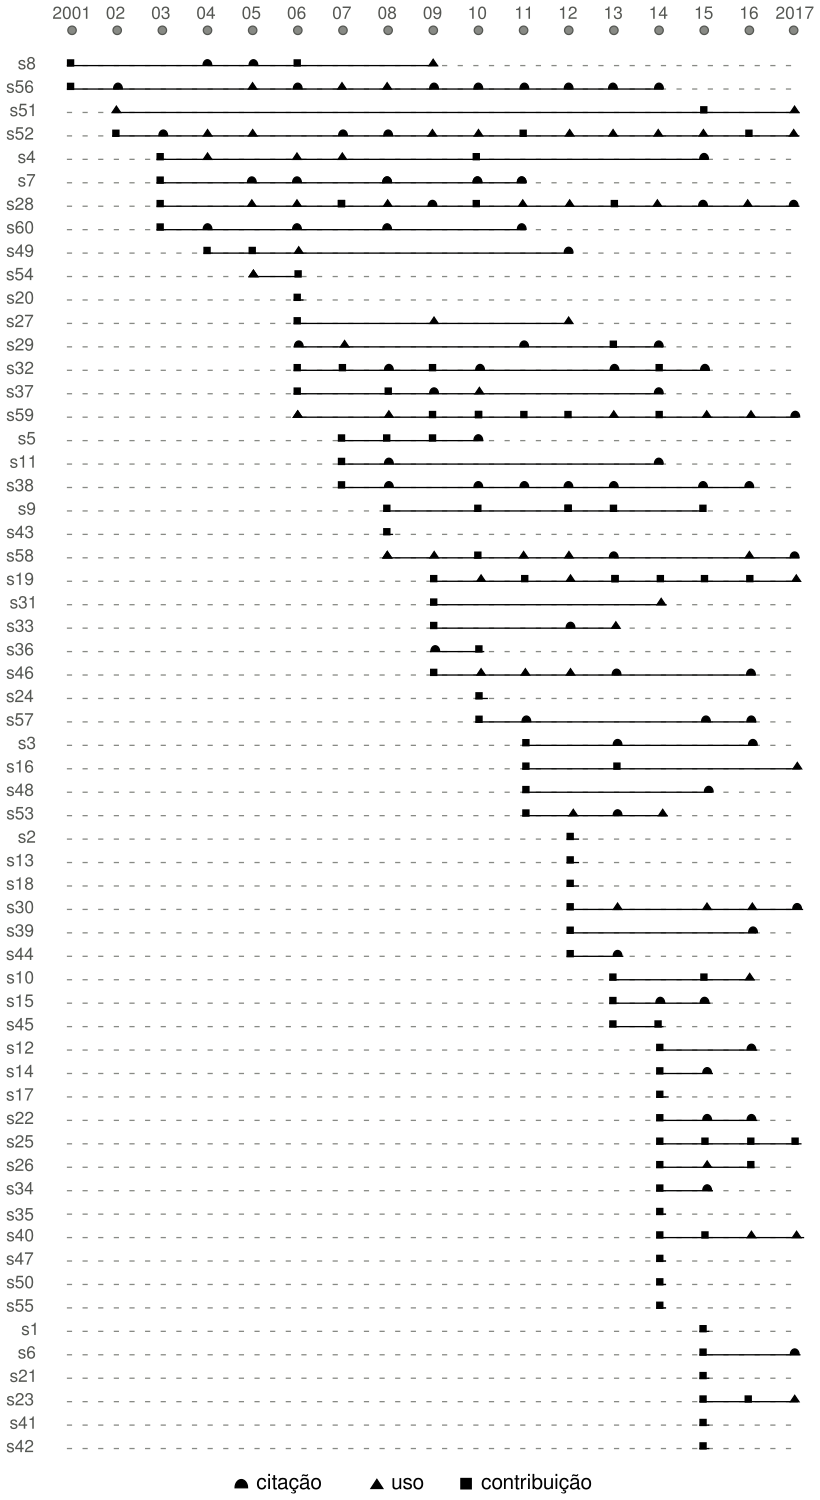
\includegraphics[scale=0.6]{imagens/mentions-timeline.png}
  \caption{Linha do tempo de menções (uso e contribuição) aos projetos nas bases ACM e IEEE.}
  \label{mentions-timeline}
\end{figure}

% }}}

% Hypothesis rejection
\section{Interpretação dos Resultados} \label{estudo2:interpretacao} % {{{

\subsection{Q1 - \EstudoDoisQuestaoUm}

Os \SoftwareCount \ projetos de software acadêmico de análise estática
publicados nas conferências ASE e SCAM são mencionados \ScreeningCount \ vezes
em \ScreeningUniqueCount \ artigos distintos, estas menções foram encontradas
em buscas nas bases ACM e IEEE realizadas entre os meses de Julho e Agosto de
2017.

Entre todas as menções emergiu três tipos distintos em relação ao nível de
contribuição ao ecossistema dos projetos, Cita, Usa e Contribui. A maior parte
das menções encontradas é do tipo Cita (\CiteCount \ menções), em seguida
o tipo de menção Usa com \UseCount \ ocorrências, e por fim, com menor número,
o tipo de menção Contribui com \ContributeCount \ ocorrências.

\subsection{Q2 - \EstudoDoisQuestaoDois}

Encontramos \UseCount \ menções usando os projetos como apoio metodológico para
coleta ou análise de dados, como objeto de estudo, ou como ponto de partida
para implementação de outras soluções de pesquisa.

Estas menções do tipo Uso estão associadas a 26 dos \SoftwareCount \ projetos
de software, indicando que menos da metade dos projetos de software acadêmico
de análise estática publicados nas conferências ASE e SCAM são utilizados em
pesquisas nas bases ACM e IEEE.

\subsection{Q3 - \EstudoDoisQuestaoTres}

Encontramos \ContributeCount \ menções contribuindo com os projetos, este total
inclui os artigos publicando os projetos de software pela primeira vez, ou
seja, inclui os artigos que deram origem ao conjunto de \SoftwareCount \
projetos de software registrados nos arquivos \texttt{paper.bib}.

Ao analisar apenas contribuições posteriores a publicação inicial
do projeto, ou seja, artigos e estudos contribuindo com código
fonte aos projetos após a sua publicação inicial, encontramos
\ContributeStudyDoisCount \ menções a um conjunto de
\ContributeStudyDoisSoftware \ projetos de software.

Ou seja, apenas 28\% dos projetos (\texttt{s10}, \texttt{s19}, \texttt{s23}, \texttt{s25}, \texttt{s26}, \texttt{s28}, \texttt{s32}, \texttt{s37}, \texttt{s4}, \texttt{s40}, \texttt{s45}, \texttt{s49}, \texttt{s5}, \texttt{s52}, \texttt{s59}, \texttt{s67}, \texttt{s8}, \texttt{s9}
)
recebem contribuição em código fonte de estudos após a publicação inicial, ao
menos entre estudos encontrados nas bases ACM e IEEE.

%O GRT recebe uma grande contribuição além da publicação inicial criando o projeto,
%é o único, todos os outros recebem contribuições de peso apenas na criação, ou seja,
%no paper original publicando o projeto pela primeira vez.

%Os projetos tiveram contribuições em código em publicações posteriores aos
%artigos inicias publicando o software?

%Quantos autores novos além dos autores originais/iniciais do projeto
%foram encontrados contribuindo com os projetos?

%

\begin{longtable}{ l *{17}{c} }
\caption{Número de publicações mencionando contribuição por ano (de 2001 até 2017).}
\label{contributors-table} \\
  \hline
  \hhline{ l *{17}{c} |}
  \endfirsthead
  \hhline{ l *{17}{c} |}
  \hline
  \textbf{Projeto} & 01 & 02 & 03 & 04 & 05 & 06 & 07 & 08 & 09 & 10 & 11 & 12 & 13 & 14 & 15 & 16 & 17 \\
  \hline
  \hhline{ l *{17}{c} |}
  \endhead
  \hhline{------------------}
  \multicolumn{17}{c}{continua na próxima página} \\
  \hhline{------------------} \endfoot
  \hhline{------------------} \endlastfoot
  \textbf{Projeto} & 01 & 02 & 03 & 04 & 05 & 06 & 07 & 08 & 09 & 10 & 11 & 12 & 13 & 14 & 15 & 16 & 17 \\
  \hline
    2LS &
      - &
      - &
      - &
      - &
      - &
      - &
      - &
      - &
      - &
      - &
      - &
      - &
      - &
      - &
      c &
      - &
      - \\
    AccessAnalysis &
      - &
      - &
      - &
      - &
      - &
      - &
      - &
      - &
      - &
      - &
      - &
      c &
      - &
      - &
      - &
      - &
      - \\
    APIExample &
      - &
      - &
      - &
      - &
      - &
      - &
      - &
      - &
      - &
      - &
      c &
      - &
      m &
      - &
      - &
      m &
      - \\
    BEG &
      - &
      - &
      c &
      u &
      - &
      u &
      u &
      - &
      - &
      c &
      - &
      - &
      - &
      - &
      m &
      - &
      - \\
    ccJava &
      - &
      - &
      - &
      - &
      - &
      - &
      c &
      c &
      c &
      c &
      - &
      - &
      - &
      - &
      - &
      - &
      - \\
    CIVL &
      - &
      - &
      - &
      - &
      - &
      - &
      - &
      - &
      - &
      - &
      - &
      - &
      - &
      - &
      c &
      - &
      m \\
    CodeBoost &
      - &
      - &
      c &
      - &
      m &
      m &
      - &
      m &
      m &
      m &
      m &
      m &
      m &
      - &
      m &
      - &
      - \\
    CSL &
      c &
      - &
      - &
      m &
      m &
      c &
      - &
      - &
      u &
      - &
      - &
      - &
      - &
      - &
      - &
      - &
      - \\
    CPA+ &
      - &
      - &
      - &
      - &
      - &
      - &
      - &
      c &
      - &
      c &
      - &
      c &
      c &
      - &
      c &
      - &
      - \\
    CSeq &
      - &
      - &
      - &
      - &
      - &
      - &
      - &
      - &
      - &
      - &
      - &
      - &
      c &
      - &
      c &
      u &
      - \\
    DDVerify &
      - &
      - &
      - &
      - &
      - &
      - &
      c &
      m &
      - &
      - &
      - &
      - &
      - &
      m &
      - &
      - &
      - \\
    Derailer &
      - &
      - &
      - &
      - &
      - &
      - &
      - &
      - &
      - &
      - &
      - &
      - &
      - &
      c &
      - &
      m &
      - \\
    Diagnosys &
      - &
      - &
      - &
      - &
      - &
      - &
      - &
      - &
      - &
      - &
      - &
      c &
      - &
      - &
      - &
      - &
      - \\
    DOMPLETION &
      - &
      - &
      - &
      - &
      - &
      - &
      - &
      - &
      - &
      - &
      - &
      - &
      - &
      c &
      m &
      - &
      - \\
    DRC &
      - &
      - &
      - &
      - &
      - &
      - &
      - &
      - &
      - &
      - &
      - &
      - &
      c &
      m &
      m &
      - &
      - \\
    e-munity &
      - &
      - &
      - &
      - &
      - &
      - &
      - &
      - &
      - &
      - &
      - &
      - &
      - &
      c &
      - &
      - &
      - \\
    EJB &
      - &
      - &
      - &
      - &
      - &
      - &
      - &
      - &
      - &
      - &
      c &
      - &
      m &
      - &
      - &
      - &
      u \\
    Error Prone &
      - &
      - &
      - &
      - &
      - &
      - &
      - &
      - &
      - &
      - &
      - &
      c &
      - &
      - &
      u &
      - &
      - \\
    ESBMC &
      - &
      - &
      - &
      - &
      - &
      - &
      - &
      - &
      c &
      u &
      c &
      u &
      c &
      c &
      c &
      c &
      u \\
    ETXL &
      - &
      - &
      - &
      - &
      - &
      c &
      - &
      - &
      - &
      - &
      - &
      - &
      - &
      - &
      - &
      - &
      - \\
    FaultBuster &
      - &
      - &
      - &
      - &
      - &
      - &
      - &
      - &
      - &
      - &
      - &
      - &
      - &
      - &
      c &
      - &
      - \\
    Flowgen &
      - &
      - &
      - &
      - &
      - &
      - &
      - &
      - &
      - &
      - &
      - &
      - &
      - &
      c &
      m &
      m &
      - \\
    GRT &
      - &
      - &
      - &
      - &
      - &
      - &
      - &
      - &
      - &
      - &
      - &
      - &
      - &
      m &
      c &
      c &
      u \\
    GUIZMO &
      - &
      - &
      - &
      - &
      - &
      - &
      - &
      - &
      - &
      c &
      - &
      - &
      - &
      - &
      - &
      - &
      - \\
    GumTree &
      - &
      - &
      - &
      - &
      - &
      - &
      - &
      - &
      - &
      - &
      - &
      - &
      - &
      c &
      u &
      u &
      c \\
    HUSACCT &
      - &
      - &
      - &
      - &
      - &
      - &
      - &
      - &
      - &
      - &
      - &
      - &
      - &
      c &
      u &
      c &
      - \\
    Indus &
      - &
      - &
      - &
      - &
      - &
      c &
      - &
      - &
      u &
      - &
      - &
      u &
      - &
      - &
      - &
      - &
      - \\
    JastAdd &
      - &
      - &
      m &
      - &
      u &
      u &
      c &
      c &
      m &
      c &
      u &
      u &
      c &
      u &
      m &
      u &
      m \\
    JFlow &
      - &
      - &
      - &
      - &
      - &
      m &
      u &
      - &
      - &
      - &
      m &
      - &
      c &
      m &
      - &
      - &
      - \\
    JstereoCode &
      - &
      - &
      - &
      - &
      - &
      - &
      - &
      - &
      - &
      - &
      - &
      c &
      u &
      - &
      u &
      u &
      m \\
    Jtop &
      - &
      - &
      - &
      - &
      - &
      - &
      - &
      - &
      c &
      - &
      - &
      - &
      - &
      u &
      - &
      - &
      - \\
    Bogor/Kiasan &
      - &
      - &
      - &
      - &
      - &
      c &
      c &
      m &
      c &
      m &
      - &
      - &
      m &
      c &
      m &
      - &
      - \\
    Loopfrog &
      - &
      - &
      - &
      - &
      - &
      - &
      - &
      - &
      c &
      - &
      - &
      m &
      u &
      - &
      - &
      - &
      - \\
    Lotrack &
      - &
      - &
      - &
      - &
      - &
      - &
      - &
      - &
      - &
      - &
      - &
      - &
      - &
      c &
      m &
      - &
      - \\
    MPAnalyzer &
      - &
      - &
      - &
      - &
      - &
      - &
      - &
      - &
      - &
      - &
      - &
      - &
      - &
      c &
      - &
      - &
      - \\
    MSP &
      - &
      - &
      - &
      - &
      - &
      - &
      - &
      - &
      m &
      c &
      - &
      - &
      - &
      - &
      - &
      - &
      - \\
    mygcc &
      - &
      - &
      - &
      - &
      - &
      c &
      - &
      c &
      m &
      u &
      - &
      - &
      - &
      m &
      - &
      - &
      - \\
    PARSEWeb &
      - &
      - &
      - &
      - &
      - &
      - &
      c &
      u &
      - &
      m &
      m &
      m &
      m &
      - &
      m &
      m &
      - \\
    PAT &
      - &
      - &
      - &
      - &
      - &
      - &
      - &
      - &
      - &
      - &
      - &
      c &
      - &
      - &
      - &
      m &
      m \\
    PHP AiR &
      - &
      - &
      - &
      - &
      - &
      - &
      - &
      - &
      - &
      - &
      - &
      - &
      - &
      c &
      c &
      u &
      u \\
    protopurity &
      - &
      - &
      - &
      - &
      - &
      - &
      - &
      - &
      - &
      - &
      - &
      - &
      - &
      - &
      c &
      - &
      - \\
    Pseudogen &
      - &
      - &
      - &
      - &
      - &
      - &
      - &
      - &
      - &
      - &
      - &
      - &
      - &
      - &
      c &
      - &
      - \\
    PtYasm &
      - &
      - &
      - &
      - &
      - &
      - &
      - &
      c &
      - &
      - &
      - &
      - &
      - &
      - &
      - &
      - &
      - \\
    PuMoC &
      - &
      - &
      - &
      - &
      - &
      - &
      - &
      - &
      - &
      - &
      - &
      c &
      m &
      - &
      - &
      - &
      - \\
    PYTHIA &
      - &
      - &
      - &
      - &
      - &
      - &
      - &
      - &
      - &
      - &
      - &
      - &
      c &
      c &
      - &
      - &
      - \\
    ReAssert &
      - &
      - &
      - &
      - &
      - &
      - &
      - &
      - &
      c &
      u &
      u &
      u &
      m &
      - &
      - &
      m &
      - \\
    Rêve &
      - &
      - &
      - &
      - &
      - &
      - &
      - &
      - &
      - &
      - &
      - &
      - &
      - &
      c &
      - &
      - &
      - \\
    RRFinder &
      - &
      - &
      - &
      - &
      - &
      - &
      - &
      - &
      - &
      - &
      c &
      - &
      - &
      m &
      m &
      - &
      - \\
    Sapid/XML &
      - &
      - &
      - &
      c &
      c &
      u &
      - &
      - &
      - &
      - &
      - &
      m &
      - &
      - &
      - &
      - &
      - \\
    Sonar Qube Plug-in &
      - &
      - &
      - &
      - &
      - &
      - &
      - &
      - &
      - &
      - &
      - &
      - &
      - &
      c &
      - &
      - &
      - \\
    SPARTA &
      - &
      u &
      - &
      - &
      - &
      - &
      - &
      - &
      - &
      - &
      - &
      - &
      - &
      - &
      c &
      - &
      u \\
    srcML &
      - &
      m &
      m &
      u &
      u &
      - &
      m &
      m &
      u &
      u &
      c &
      u &
      u &
      u &
      u &
      c &
      u \\
    SWAT &
      - &
      - &
      - &
      - &
      - &
      - &
      - &
      - &
      - &
      - &
      c &
      u &
      m &
      u &
      - &
      - &
      - \\
    TACLE &
      - &
      - &
      - &
      - &
      u &
      c &
      - &
      - &
      - &
      - &
      - &
      - &
      - &
      - &
      - &
      - &
      - \\
    TEBA &
      - &
      - &
      - &
      - &
      - &
      - &
      - &
      - &
      - &
      - &
      - &
      - &
      - &
      c &
      - &
      - &
      - \\
    TestEra &
      c &
      m &
      - &
      u &
      m &
      m &
      u &
      u &
      m &
      m &
      m &
      m &
      m &
      m &
      - &
      - &
      - \\
    Vdiff &
      - &
      - &
      - &
      - &
      - &
      - &
      - &
      - &
      - &
      c &
      m &
      - &
      - &
      - &
      m &
      m &
      - \\
    WALA &
      - &
      - &
      - &
      - &
      - &
      - &
      - &
      u &
      u &
      c &
      u &
      u &
      m &
      - &
      - &
      u &
      m \\
    Wrangler &
      - &
      - &
      - &
      - &
      - &
      u &
      - &
      u &
      c &
      c &
      c &
      c &
      u &
      c &
      u &
      u &
      m \\
    XOgastan &
      - &
      - &
      c &
      m &
      - &
      m &
      - &
      m &
      - &
      - &
      m &
      - &
      - &
      - &
      - &
      - &
      - \\
  \hline
\end{longtable}



%A comparação entre os nomes do autores passou antes pela normalização
%no formato de representação, visto que cada artigo utiliza um formato
%de nome diferente, transformamos, por exemplo, ``Bajaj, Kon'' em ``Bajaj K.'',
%``Costa, Kim A.'' em ``Costa K. A.'', ``Rajan, Sreeranga P.'' em ``Rajan S. P.'',
%``Pol, Jaco van de'' em ``Pol J. van de'', ``Zijiang Yang'' em ``Yang Z.'',
%e assim comparamos dois nomes considerando que cada um destes nomes representa,
%de forma única, um autor.

% }}}

\section{Ameaças à validade} % {{{

A inspeção manual dos artigos na revisão de literatura em busca de caracterizar
as menções e seus tipos foi realizada apenas pelo autor desta dissertação, isto
pode levar a inconsistência na interpretação das menções em relação aos projetos
investigados, uma vez que a inspeção é realizada num processo estritamente
subjetivo, esta ameaça não foi tratada.

A busca realizada apenas nas bases da ACM e IEEE pode ter deixado fora dos
resultados possíveis artigos mencionando os projetos investigados, uma vez que
é possível que existam publicações não indexadas por estas bases, Apesar disso,
estas duas bases possuem grande relevância para a área de Engenharia de
Software, de forma que esta ameaça não prejudica as conclusões do estudo, uma
vez que todas as conclusões estão estreitamente associadas a este recorte e não
sugerimos serem generalizadas.

É possível que a falta de contribuição aos projetos seja um reflexo da
relevância do estudo onde foram publicados, ou seja, projetos publicados em
artigos com pouca relevância, com pouca visibilidade, pode, eventualmente,
atrair pouca atenção, consequentemente receber pouca contribuição. No entanto,
a relevância do software não está necessariamente associada a relevância do
estudo, é possível que projetos de software extremamente úteis e relevantes
para a comunidade científica tenham sido publicados em artigos com pouca ou
nenhuma relevância. Dessa forma esta ameaça não impacta negativamente as nossas
conclusões, uma vez que estamos interessados em capturar quanta colaboração há
entre os projetos, do ponto de vista de sua utilidade para o corpo científico
como um todo.

% }}}

\section{Conclusões} \label{estudo2:conclusoes} % {{{

Este estudo inspecionou \SearchUniqueCount \ artigos encontrados nas bases ACM
e IEEE através de busca avançada usando características de \SoftwareCount \
projetos de software acadêmico de análise estática. Durante a inspeção foi
encontrada \ScreeningCount \ menções distribuídas entre os tipos Cita, Usa ou
Contribui.

Estes tipos emergiram da análise sobre como os projetos são mencionados nos
artigos, entre todas as menções, \CiteCount \ são do tipo Cita, \UseCount \ Usa
e \ContributeCount \ Contribui. As menções do tipo Contribui incluem os artigos
iniciais publicando os projetos pela primeira vez pelos autores originais,
ao excluir estes artigos, encontramos apenas \ContributeStudyDoisCount \ menções
do tipo Contribui.

Este número de menções está relacionada a apenas 28\% do conjunto total de
projetos, isto indica que não parece haver uma prática de contribuição entre os
pesquisadores em relação a código fonte dos seus projetos de software, ao menos
no contexto de análise estática.

%Identificou-se que uma quantidade mínima de artigos contribui com código fonte aos
%projetos estudados nesta pesquisa, apenas 28\% dos projetos recebem contribuições
%após a contribuição inicial publicada pelos seus autores. Este pequeno conjunto
%recebeu \ContributeStudyDoisCount \ contribuições em código fonte, 

Não encontramos relação entre a disponibilidade de download, forma de
distribuição ou linguagem de programação e o número de menções, entre os
projetos com maior contribuição temos Java, C, Erlang e Rascal.

Acreditamos que o número de menções, seja de Uso ou Contribuição, está
intimamente ligado a relevância prática do projeto e aos atributos de
qualidade, como, usabilidade, portabilidade, facilidade de instalação, entre
outros. No entando não investigamos estes atributos neste estudo.

Acreditamos fortemente que manutenibilidade, ou seja, o esforço necessário para
realizar alteraçoes no código fonte de um software, está intrinsicamente
relacionado ao número de contribuições destes projetos. Desta forma, planejamos
um terceiro estudo para investigar este aspecto de qualidade entre os projetos
estudados.

%ou ao menos um subconjunto deles, já que uma parte não está disponível em
%código fonte e o estudo que faremos será através da análise deste artefato.

%Entretanto, acredita-se que um atributo de qualidade externa, como
%manutenibilidade por exemplo, tem relação com o número de contribuição, uma vez
%que a facilidade de contribuição está diretamente relacionada a facilidade de
%intervenção e manutenção no código fonte destes projetos.

%FALTA uma síntese aqui. 
%Este estudo ...
%Resultados mostram que ...
%Algumas tendências emergiram a partir da leitura ...
%
%Planejamos fazer outro estudo ... 

% }}}

% o artigo com resumo do RESER 2011 diz \cite{knutson2010report}:
% 4) Re-
% search tools are either not available or not usable, so precise
% replication is impractical [1, 2, 8, 18, 19].

%Acesso ao software
%
%5º Princípio da citação ao softwares, Acessibilidade:
%
%``citações aos softwares devem permitir e facilitar acesso ao software,
%metadados, documentação, dados e outros materiais necessários tanto
%para humanos quanto para máquinas se informar do referido software''
%
%Não significa que o software deva estar disponível gratuitamente, mas que
%os metadados devem prover informação suficiente para que o software seja
%acessado. Se o software é livre, os metadados devem prover um identificador
%que pode ser resolvido para uma URL apontando para a versão específica
%do software sendo citado.
%
%Pra softwares comerciais, os metadados devem ainda prover informações sobre
%como acessa o software, mas pode ser um número de telefone da empresa que
%vende o software ou o link para um site que venda o software
%
%\cite{smith2016software}
%
%5. Accessibility: Software citations should facilitate access to the software itself and to its

%\subsection{Autoria das menções aos projetos de software de análise estática}

%das bibliotecas digitais, temos para cada um dos artigos todos os seus
%metadados,. Os autores de
%cada uma das menções ao software, por exemplo, serão utilizados na fase de
%análise para calcular o quanto de autores novos começaram a publicar sobre
%certo software acadêmico.

%Os dados coletados sobre as menções a cada software foram acrescentados com uma
%nova informação calculada a partir da autoria de cada artigo mencionando o
%software, estamos considerando que todos os autores de um certo artigo tem o
%mesmo peso em relação a menção ao software naquele estudo, mesmo sabendo que não
%é raro que cientistas trabalhando em conjunto apresentem níveis diferentes de
%domínio sobre cada parte da pesquisa.

%Os autores originais do primeiro artigo publicando sobre software, na maior
%parte dos casos é o mesmo paper selecionado no estudo anterior que deu origem
%ao conjunto de projetos, são considerados os autores originais do projeto, a
%partir desta primeira publicação cada artigo mencionando o software indica a
%entrada de novos atores no ecossistema daquele software.

%Foi coletado então para cada artigo em relação aos autores o quanto são
%autores novos, e classificamos em termos de todos os autores do estudo
%são novos, se todos já publicaram sobre o software anteriormente, ou se
%nenhum dos autores jamais publicou sobre aquele software anteriormente, A Tabela
%\ref{esquema-de-autoria} apresenta em detalhes este esquema.

%representado quantos novos atores foram incluídos
%no ecossistema daquele software, isto foi feito comparando o conjunto de autores
%da publicaçao com o conjunto acumulado de todos os autores anteriores, 
%podendo assumir um dos valores da Tabela \ref{coding-scheme-author}.

%\begin{table}[h]
%\caption{Esquema para classificação de autoria de menções aos projetos de software acadêmico.}
%\centering
%\begin{tabular}{ l c p{8cm} }
%  \hline
%  Novos atores no ecossistema & Peso & Explicação \\
%  \hline
%  Nenhum    & 0.5  & Nenhum dos autores jamais publicou sobre o software \\
%  Parte     & 0.25 & Uma parte dos autores já publicou sobre o software em anos anteriores \\
%  Todos     & 0.1  & Todos os autores já publicaram sobre o software em anos anteriores \\
%  Criadores & 0    & São os primeiros autores a publicar sobre o software \\
%  \hline
%\end{tabular}
%\label{esquema-de-autoria}
%\end{table}

%Estes dados foram calculados com base nos metadados já coletados anteriormente
%dispníveis nos arquivos BibTeX com as menções à cada projeto, tratamos os nomes
%dos autores para utilizar o mesmo formato, já que os artigos variam em relação
%ao padrão de nomes dos autores.

%Com os nomes dos autores normalizados comparamos e caso tenham a mesma string
%consideramos que trata-se de um mesmo pesquisador, os nomes iguals são
%considerados como sendo a mesma pessoa. Avaliamos cada artigo em ordem
%cronológica comparando os autores com relação a todos os autores anteriores.

%Este processo foi realizado automaticamente com um script escrito durante este
%trabalho de pesquisa, os dados resultantes são armazenados de volta nos
%arquivos BibTeX.

%\subsection{Autoria das menções aos projetos de software de análise estática}

% nao vou mais analisar nenhum dado de autoria, apenas numero de citacoes e tipo!!!
%
\begin{longtable}{ l c c }
\caption{Número de autores únicos mencionando os projetos de software.}
\label{authorship-table} \\
  \hline
  \hhline{ l c c |}
  \endfirsthead
  \hhline{ l c c |}
  \hline
  \textbf{Nome do software} & {\bf Autores únicos} & {\bf Menções} \\
  \hline
  \hhline{ l c c |}
  \endhead
  \hhline{---}
  \multicolumn{3}{c}{continua na próxima página} \\
  \hhline{---} \endfoot
  \hhline{---} \endlastfoot
  \textbf{Nome do software} & {\bf Autores únicos} & {\bf Menções} \\
  \hline
   2LS & 5 & 1 \\
   AccessAnalysis & 2 & 2 \\
   APIExample & 15 & 4 \\
   BEG & 11 & 9 \\
   ccJava & 6 & 5 \\
   CIVL & 24 & 6 \\
   CodeBoost & 36 & 15 \\
   CSL & 12 & 6 \\
   CPA+ & 11 & 5 \\
   CSeq & 13 & 5 \\
   DDVerify & 9 & 3 \\
   Derailer & 2 & 2 \\
   Diagnosys & 4 & 1 \\
   DOMPLETION & 3 & 2 \\
   DRC & 10 & 5 \\
   e-munity & 5 & 1 \\
   EJB & 8 & 3 \\
   Error Prone & 9 & 2 \\
   ESBMC & 119 & 42 \\
   ETXL & 2 & 1 \\
   FaultBuster & 5 & 1 \\
   Flowgen & 8 & 3 \\
   GRT & 25 & 10 \\
   GUIZMO & 3 & 1 \\
   GumTree & 68 & 19 \\
   HUSACCT & 10 & 7 \\
   Indus & 7 & 4 \\
   JastAdd & 107 & 45 \\
   JFlow & 21 & 7 \\
   JstereoCode & 24 & 8 \\
   Jtop & 5 & 2 \\
   Bogor/Kiasan & 43 & 16 \\
   Loopfrog & 14 & 5 \\
   Lotrack & 5 & 2 \\
   MPAnalyzer & 2 & 1 \\
   MSP & 5 & 2 \\
   mygcc & 21 & 7 \\
   PARSEWeb & 73 & 24 \\
   PAT & 7 & 3 \\
   PHP AiR & 8 & 9 \\
   protopurity & 4 & 1 \\
   Pseudogen & 8 & 1 \\
   PtYasm & 5 & 2 \\
   PuMoC & 2 & 2 \\
   PYTHIA & 3 & 2 \\
   ReAssert & 38 & 13 \\
   Rêve & 5 & 1 \\
   RRFinder & 12 & 3 \\
   Sapid/XML & 5 & 5 \\
   Sonar Qube Plug-in & 5 & 1 \\
   SPARTA & 15 & 4 \\
   srcML & 99 & 40 \\
   SWAT & 6 & 4 \\
   TACLE & 3 & 3 \\
   TEBA & 2 & 1 \\
   TestEra & 39 & 23 \\
   Vdiff & 15 & 5 \\
   WALA & 37 & 11 \\
   Wrangler & 61 & 33 \\
   XOgastan & 17 & 5 \\
  \hline
  {\bf Total} & 983 & 456 \\
\end{longtable}



%bem como identificar quais tipos de menções e 
%publicados nas conferências de Engenharia de Software ASE e SCAM são
%mencionados em publicações nas bases ACM e IEEE.

%e pdf,
%estes resultados devem incluir ao menos os artigos selecionados
%no estudo anterior onde os projetos foram encontrados, já que tais artigos são
%o caso mínimo de resultado desejado nesta fase de busca. 

%de cada projeto, sem duplicidade, cada artigo receberá um ID único, este ID
%será utilizado nas etapas seguintes.

%, e um com um merge destes dois mantendo resultados únicos sem
%duplicidade.

%Para cada software, os resultados foram agrupados
%num arquivo único, sem duplicidade entre os resultados trazidos por cada base
%bibliográfica. O arquivo de metadados de cada software contém informações sobre
%o artigo, autores, ano de publicação, conferência, jornal, etc. Os artigos
%também foram armazenados localmente, no formato pdf para serem analisados na
%triagem.

%A busca avançada na base ACM (Figura \ref{advanced-search-acm}) não necessita
%marcar nenhum campo adicional além do próprio campo texto onde deve-se entrar
%com a string de busca de cada projeto. Para cada projeto de software são construídas duas strings, uma para busca na
%base da ACM, outra para busca na base IEEE.

%buscamos inicialmente usando apenas o nome do software, analisamos o número total
%de resultados e os títulos destes resultados, quando o número de resultados for
%muito grande, acima de XXX, e os títulos não aparentavam ser estudos com relação
%aos projetos, incluímos mais características, como por exemplo, parte da descrição
%do software, ou parte da URL, autores, etc.

%avançada realizada para cada string, os artigos são
%inspecionados manualmente em busca de confirmar se fazem realmente menção ao
%projeto.

%Neste estudo as menções  pesquisadas nas bases ACM e IEEE teve como critério
%mínimo a identificação do projeto de software através do nome, ou seja, não
%buscamos publicações que não fizessem menção ao nome do software.

%A inspeção tem como objetivo selecionar os artigos relevantes para este estudo,
%mantendo apenas aqueles com menção ao nome do software, seja a menção em
%formato de citação formal ou informal.

%o uma escala de pesos, onde o último tipo
%de menção inclui implicitamente os tipos de menor peso, este peso representa
%o nível de contribuição da menção ao ecossistema do projeto de software.

%Um tipo de menção com maior peso inclui implicitamente o tipo de menção de
%menor peso, e assim sucessivamente.

%, estando
%incluído nestes conjuntos ao menos os próprios artigos que deram origem ao
%conjunto de projetos utilizados como objeto de estudo neste trabalho.

%menções a eles nas bases do ACM e IEEE, temos o tipo de cada menção, se
%contribuiu com o projeto, se foi avaliado, ou apenas citado como referência, os
%artigos selecionados no estudo anterior que deram origem ao conjunto de
%projetos de software estão incluídos nestes resultados.

%Todos estes scripts estão disponíveis no repositório desta dissertação e foram desenvolvidos
%utilizando a a linguagem de
%programação Perl\footnote{\url{http://perl.org}} com o auxílio dos
%módulos Modern::Perl\footnote{\url{http://metacpan.org/pod/Modern::Perl}},
%YAML\footnote{\url{http://metacpan.org/pod/YAML}},
%Mojo::Template\footnote{\url{http://metacpan.org/pod/Mojo::Template}},
%Text::BibTeX\footnote{\url{http://metacpan.org/pod/Text::BibTeX}} e
%List::Util\footnote{\url{http://metacpan.org/pod/List::Util}}.
%A maior parte da lógica foi implementada no arquivo
%\texttt{lib/Dissertacao.pm} com objetivo de reduzir repetição de código e
%proporcionar reuso.

%Definimos uma identificação única para cada um dos 60 projetos de software
%utilizando o próprio arquivo \texttt{software.yml} através do campo
%\texttt{id:} seguindo o padrão \texttt{s + número}, exemplo, \texttt{s1},
%\texttt{s2}, \texttt{s3}, \texttt{s4}, ..., \texttt{s60}, cada projeto de software
%recebeu um id.

%Definimos um novo campo neste mesmo arquivo para coleta das menções, fazendo
%referência ao ID do artigo mencionando o software, com os campos ... cada artigo
%encontrado na revisão de literatura também receberá um ID, desta forma será possível
%relacionar projetos e artigos através das menções.
%
%...

%esquema
%para cada artigo será extraído qual o
%tipo de menção é feito ao software, quando o artigo menciona o software
%diversas vezes deve ser adotado o tipo de menção de maior relevância para este
%estudo, onde o tipo de menção de maior peso inclui implicitamente os tipos
%menores.

%Um documento
%CSV com todas as strings de busca pode ser encontrado no repositório desta
%dissertaçao no arquivo \texttt{documents/search-strings.csv}.

%Para auxiliar a definição da identificação para cada artigo implementamos o script \texttt{bin/ids}, este script

%, este arquivo contém os metadados de todos os
%artigos encontrados pelas strings de busca de cada projeto nas bases ACM e IEEE
%com um id único no formato 

%cada item uma identificação única, esta identificação será utilizada nas etapas
%seguintes da revisão de literatura para relacionar os projeto com os
%artigos através das menções identificadas.
%único, localizado em

%dois arquivos para cada projeto de software, um contendo os resultados da busca na base ACM -- .
%arquivo único são

%de cada artigo é realizada com o auxílio da funcionalidade de busca
%do leitor de pdf utilizado neste estudo\footnote{Utilizamos software Evince v3.22.1}
%utilizado para leitura dos artigos, com o auxílio da busca encontramos cada
%ocorrência ao nome do software tomando nota a confirmação sobre a menção
%encontrada.

%Esta informação foi armazenada no próprio arquivo BibTeX num campo adicional
%aos demais campos dos metadados do artigo; ao final, temos os metadados do
%artigo como, título, autores, ano de publicação, etc, e também uma indicação se
%o artigo cita realmente o software.

%\texttt{references.yml} de cada projeto onde iremos anotar e coletar os dados
%da triagem, além do template utilizado como modelo para estes arquivos
%implementamos também 

%cada artigo presente no arquivo \texttt{documents/references.bib} será
%inspecionado, os dados coletados neste passo serão armazenados no arquivo
%\texttt{is\_software\_mentioned} deve ser criado com os valores \texttt{yes} ou
%\texttt{no} indicando se o artigo menciona ou não o projeto.

%Implementamos scripts para transformar os dados da busca em formato BibTeX para
%arquivos no formato YML pois a coleta e inspeção dos artigos serão registrados
%em arquivos YML para cada projeto de software. Estes scripts recebem como entrada
%os resultados da busca de todos os projetos e geram como saída os arquivos \texttt{references.bib}
%e \texttt{references.yml} para cada projeto.

%no arquivo
%\texttt{references.yml} no campo \texttt{review} sobre como o software é
%mencionado naquele artigo.

%para cada projeto, a Listagem \ref{references-yml} apresenta um exemplo do
%trecho do YML para armazenar a extração dessas informações.

%Os dados extraídos são armazenados no arquivo \texttt{references.yml} de
%cada projeto, sendo atualizado com a inclusão de um novo campo indicando o tipo
%de menção do artigo ao software, \texttt{mention\_type},

%para utilizar na etapa de análise. Implementamos também templates para gerar arquivos em
%formato TeX para posterior inclusão na seção de coleta onde apresentaremos os dados
%coletados.

%Os dados armazenados em arquivos
%YAML e BibTeX são carregados em estruturas em memória através de um script
%escrito em linguagem Perl e repassados para templates processados para exibir
%os dados neste texto, em arquivos TeX, CSV, etc. A Figura \ref{estudo2-fluxograma}
%apresenta o fluxo de coleta, análise e transformação dos dados.

%A lista completa com autores, título e ano de publicação com todos os
%\SearchUniqueCount \ resultados pode ser consultado no arquivo
%\texttt{documents/search.md} no repositório desta dissertação.

%Alguns artigos fazem menção a mais de 1 projeto, fizemos o download de cada
%artigo e armazenamos os metadados em formato BibTeX nos arquivos \texttt{acm.bib}
%e \texttt{ieee.bib} para cada projeto de software.

%Uma tabela no formato CSV com todos os artigos e projetos, indicando quando há
%relação entre eles através de menção pode ser encontrada no repositório desta
%dissertação no arquivo \texttt{documents/references.csv}, neste arquivo todos
%os artigos e todos os projetos são representados e a relação entre eles é
%marcada com um \texttt{x} sempre que houver menção de um artigo para um
%software.

%Merge único de todos os arquivos BibTeX, incluindo o arquivo \texttt{paper.bib} de
%cada projeto gerado no estudo anterior apresentado no Capítulo \ref{estudo1}, um
%arquivo \texttt{documents/references.bib} foi criado contendo todas as referências
%a todos os projetos, referências únicas.

%334 artigos fazem menção aos 60 projetos.
%350 não faz menção aos projetos.

%Na sequencia adicionamos o \texttt{id} a cada artigo do
%\texttt{documents/references.bib}, este arquivo tem os metadados dos artigos
%encontrados, eles receberam ids, estes ids serão
%utilizados para relacionar o projeto ao artigo, o script \texttt{bin/ids}
%foi utilizado para automatizar esta função.

%Os scripts \texttt{bin/merge},  foram utilizados para gerar o
%\texttt{documents/references.bib} a partir dos arquivos \texttt{acm.bib},
%\texttt{ieee.bib} e \texttt{paper.bib} de cada projeto.

%tipos gerou uma escala de tipos de menção
%aos projetos de software, detalhado na 
%, com três valores
%distintos, onde o último tipo de menção com maior valor inclui todos os demais.

%A definição deste esquema foi feito através de anotações sobre onde e como o
%projeto de software é mencionado em cada artigo.
%É importante lembrar que um mesmo artigo pode mencionar
%mais de um software.

%, anotamos no campo
%\texttt{review} do arquivo \texttt{references.yml} um comentário textual livre
%resumindo de que forma o projeto de software é mencionado, caso várias menções
%seja encontrado num mesmo artigo para um dado projeto de software é feito um
%resumo total.

%Esta anotação foi feita no arquivo \texttt{references.yml} de cada projeto, nele
%foi adicionado um novo registro para cada artigo que faz menção e notas sobre a
%menção foi adicionada.

%também o tipo de menção que é feita ao software: se apenas cita como exemplo,
%se contribui com novos algoritmos e técnicas, se avalia, ou apenas descreve o
%software comparando-o com outro software.

%Coletamos as informações relacionadas a cada menção encontrada, cada um dos
%\ScreeningUniqueCount \ artigos encontrados mencionando os projetos, coletamos
%como o projeto é mencionado, encontramos \ScreeningCount \ menções aos
%projetos neste conjunto de artigos.

%para o campo \texttt{mention\_type}

%-- as strings de busca
%destes dois projetos não encontrou nenhum resultado, tanto na base ACM quanto
%na base IEEE.

%cada um, alguns tendo duas publicações na mesma época sendo uma
%publicação específica numa trilha de ferramenta, ou senndo 2 artigos
%semelhantes publicados na mesma época em conferências distintas, mas sendo os
%mesmos autores.

%Nenhum destes projetos tiveram menção após a publicação inicial do projeto,
%entre estes 14 projetos, apenas três (Diagnosys, ETXL e Rêve) estão
%indisponíveis para download, os outros 11 estão disponíveis, todos com código
%fonte, exceto o FaultBuster que está disponível apenas em formato binário.
